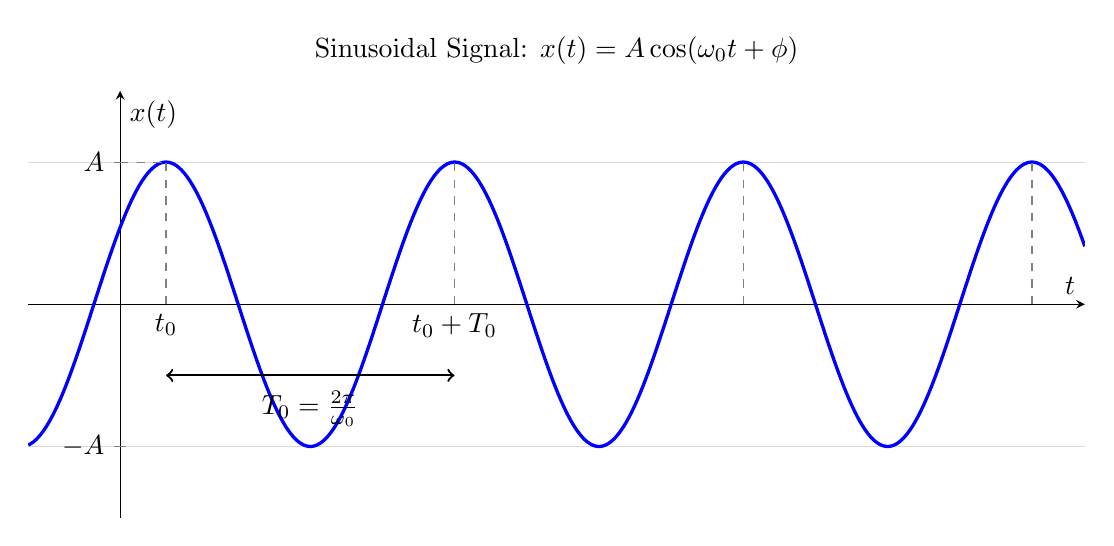
\begin{tikzpicture}
	\begin{axis}[
		% Set the overall style (wider to accommodate more cycles)
		width=15cm,
		height=7cm,
		% Title with the general function
		title={Sinusoidal Signal: $x(t) = A \cos(\omega_0 t + \phi)$},
		% Axis labels
		xlabel={$t$},
		ylabel={$x(t)$},
		% Position axes at the origin
		axis lines=middle,
		% Set axis limits to show three cycles
		xmin=-2, xmax=21,
		ymin=-1.5, ymax=1.5,
		% Disable default ticks to add custom symbolic ones
		xtick=\empty,
		ytick=\empty,
		extra y ticks={-1, 1},
		extra y tick labels={$-A$, $A$},
		% Add a grid
		grid=major,
		grid style={line width=.1pt, draw=gray!30},
		% Plotting settings
		domain=-2:21,
		samples=400, % Increased samples for a smooth curve over the larger domain
		no marks,
		]
		
		% Plot a representative cosine wave (A=1, w0=1, phi=-1 rad)
		\addplot[blue, very thick] {cos(deg(x - 1))};
		
		% --- ANNOTATIONS ---
		
		% 1. Mark the Period (T_0) between the first two peaks
		% First peak is at t=1. Period is 2*pi. Second peak is at t = 1 + 2*pi ~ 7.28
		\draw[dashed, gray] (axis cs:1,0) -- (axis cs:1,1);
		\draw[dashed, gray] (axis cs:7.28,0) -- (axis cs:7.28,1);
		
		% Add a double-arrow line to label the period
		\draw[<->, thick] (axis cs:1, -0.5) -- (axis cs:7.28, -0.5) node[midway, below=2pt] {$T_0 = \frac{2\pi}{\omega_0}$};
		
		% 2. Mark the Amplitude (A)
		% Add a guideline from the first peak to the y-axis
		\draw[dashed, gray] (axis cs:0,1) -- (axis cs:1,1);
		
		% 3. Label key time instances for the first two peaks
		\node[below] at (axis cs:1, 0) {$t_0$};
		\node[below] at (axis cs:7.28, 0) {$t_0+T_0$};
		
		% 4. Add guidelines for the subsequent peaks to show the full three cycles
		% Third peak: t = 1 + 4*pi ~ 13.57
		% Fourth peak: t = 1 + 6*pi ~ 19.85
		\draw[dashed, gray] (axis cs:13.57,0) -- (axis cs:13.57,1);
		\draw[dashed, gray] (axis cs:19.85,0) -- (axis cs:19.85,1);
		
	\end{axis}
\end{tikzpicture}